\documentclass[tikz,10pt]{standalone}
\usepackage{amsmath,amssymb,cmap,pgfplots,pgfplotstable}
\usetikzlibrary{arrows,calc,intersections}
\pgfplotsset{compat=newest}

\begin{document} 
	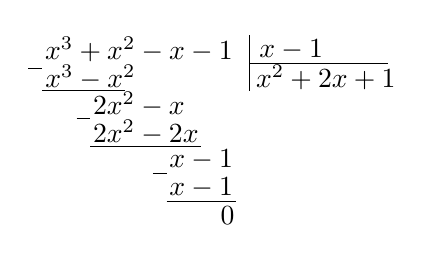
\begin{tikzpicture}
		\draw (0,0) node {$x^3 + x^2 - x - 1$};
		\draw (5.5em,0em) node {$x-1$};
		\draw (6.75em,-1em) node {$x^2+2x+1$};
		\draw (4em,-0.5em) -- (9em,-0.5em);
		\draw (4em,0.5em) -- (4em,-1.5em);
		\draw (-4em,-0.7em) -- +(0.5em,0);
		\draw (-1.75em,-1em) node {$x^3-x^2$};
		\draw (-3.5em,-1.5em) -- +(3em,0em);
		\draw (0em,-2em) node {$2x^2-x$};
		\draw (-2.25em,-2.5em) -- +(0.5em,0em);
		\draw (0.25em,-3em) node {$2x^2-2x$};
		\draw (-1.75em,-3.5em) -- +(4em,0em);
		\draw (2.25em,-4em) node {$x-1$};
		\draw (2.25em,-5em) node {$x-1$};
		\draw (0.5em,-4.5em) -- +(0.5em,0em);
		\draw (1em,-5.5em) -- +(2.5em,0em);
		\draw (3.2em,-6em) node {$0$};
	\end{tikzpicture}
\end{document}